%%%%%%%%%%%%%%%%%%%%%%%%%%%%%%%%%%%%%%%%%
% Journal Article
% LaTeX Template
% Version 1.3 (9/9/13)
%
% This template has been downloaded from:
% http://www.LaTeXTemplates.com
%
% Original author:
% Frits Wenneker (http://www.howtotex.com)
%
% License:
% CC BY-NC-SA 3.0 (http://creativecommons.org/licenses/by-nc-sa/3.0/)
%
%%%%%%%%%%%%%%%%%%%%%%%%%%%%%%%%%%%%%%%%%
%----------------------------------------------------------------------------------------
%       PACKAGES AND OTHER DOCUMENT CONFIGURATIONS
%----------------------------------------------------------------------------------------
\documentclass[paper=letter, fontsize=12pt]{article}
\usepackage[english]{babel} % English language/hyphenation
\usepackage{amsmath,amsfonts,amsthm} % Math packages
\usepackage[utf8]{inputenc}
\usepackage{float}
\usepackage{lipsum} % Package to generate dummy text throughout this template
\usepackage{blindtext}
\usepackage{algpseudocode}
\usepackage{graphicx} 
\usepackage{listings}
\usepackage{float}
\usepackage{caption}
\usepackage{multirow}
\usepackage{fullpage}
\usepackage{graphicx}
\usepackage{amsthm}
\usepackage{amssymb}
\usepackage{url}
\usepackage{amsfonts}
\usepackage{algpseudocode}
\usepackage{float}
\usepackage{mathtools} 
\usepackage{subcaption}
\usepackage[sc]{mathpazo} % Use the Palatino font
\usepackage[T1]{fontenc} % Use 8-bit encoding that has 256 glyphs
\linespread{1.05} % Line spacing - Palatino needs more space between lines
\usepackage{microtype} % Slightly tweak font spacing for aesthetics
\usepackage[hmarginratio=1:1,top=32mm,columnsep=20pt]{geometry} % Document margins
\usepackage{multicol} % Used for the two-column layout of the document
%\usepackage[hang, small,labelfont=bf,up,textfont=it,up]{caption} % Custom captions under/above floats in tables or figures
\usepackage{booktabs} % Horizontal rules in tables
\usepackage{float} % Required for tables and figures in the multi-column environment - they need to be placed in specific locations with the [H] (e.g. \begin{table}[H])
\usepackage{hyperref} % For hyperlinks in the PDF
\usepackage{lettrine} % The lettrine is the first enlarged letter at the beginning of the text
\usepackage{paralist} % Used for the compactitem environment which makes bullet points with less space between them
\usepackage{abstract} % Allows abstract customization
\renewcommand{\abstractnamefont}{\normalfont\bfseries} % Set the "Abstract" text to bold
\renewcommand{\abstracttextfont}{\normalfont\small\itshape} % Set the abstract itself to small italic text
\usepackage{titlesec} % Allows customization of titles

\renewcommand\thesection{\Roman{section}} % Roman numerals for the sections
\renewcommand\thesubsection{\Roman{subsection}} % Roman numerals for subsections

\titleformat{\section}[block]{\large\scshape\centering}{\thesection.}{1em}{} % Change the look of the section titles
\titleformat{\subsection}[block]{\large}{\thesubsection.}{1em}{} % Change the look of the section titles
\newcommand{\horrule}[1]{\rule{\linewidth}{#1}} % Create horizontal rule command with 1 argument of height
\usepackage{fancyhdr} % Headers and footers
\pagestyle{fancy} % All pages have headers and footers
\fancyhead{} % Blank out the default header
\fancyfoot{} % Blank out the default footer

\fancyhead[C]{Indiana University $\bullet$ B534 $\bullet$ Group 19 } % Custom header text

\fancyfoot[RO,LE]{\thepage} % Custom footer text
%----------------------------------------------------------------------------------------
%       TITLE SECTION
%----------------------------------------------------------------------------------------
\title{\vspace{-15mm}\fontsize{24pt}{10pt}\selectfont\textbf{Project2B: Harp Kmeans}} % Article title
\author{
\large
{\textsc{Ethan Li, Rohit Patil}}\\[2mm]
%\thanks{A thank you or further information}\\ % Your name
\normalsize {Indiana University Bloomington}\\ % Your email address
}
\date{}

%----------------------------------------------------------------------------------------
\begin{document}
\maketitle % Insert title
\thispagestyle{fancy} % All pages have headers and footers

\subsection{Descriptions}

\subsubsection{Main Steps}

\textbf{The main steps are as follows:}
{\small
\begin{center}
\begin{algorithmic}
\State Begin
\State generate data and initial centroids and write them to HDFS
\Repeat
\State configure a job
\State run the job/ do computations
\Until reach maxIteration
\State write out the results (final centroids)
\State End
\end{algorithmic}
\end{center}
}

\textbf{In each mapper task:}
{\small
\begin{center}
\begin{algorithmic}
\State Begin
\State setup, get initial values.
\State load data and centroids
\State do local computation and assign each data point to closet centroid
\State for each centroid, do local aggregation and then call allreduce
\State finalize computation and write the updated centroids back to HDFS.
\State End
\end{algorithmic}
\end{center}
}

\subsubsection{data flow}
 
 The data is being generated in memory, written to local filesystem, and then copied to HDFS. Every iteration, the data will be loaded into HDFS.\\
 The centroids are firstly generated and then wrote back to HDFS. In every iteration, they will be loaded, calculated, updated and then finally write back to HDFS. Note that in the update part, the centroids will be transferred among all mappers.
 
 
\subsection{Test}
 
To save the space, we use a small test here to get the data and final output centroids. We use the following command to run the test and got the input data at Figure~\ref{fig:data} and output centroids at Figure~\ref{fig:centroids}.\\
 
 \begin{lstlisting}
hadoop jar harp3-app-hadoop-2.6.0.jar  \
edu.iu.km.KmeansMapCollective 10 3 3 2 5 /kmeans /tmp/kmeans
 \end{lstlisting}
 
 \begin{figure}[H]  
\centering
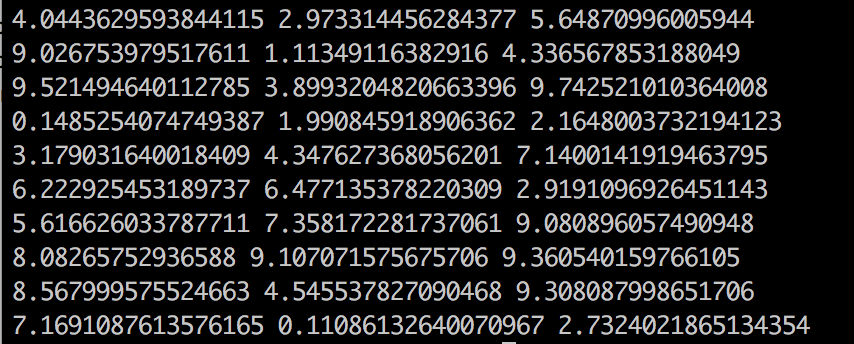
\includegraphics[width=0.9\textwidth]{data}
\caption{data}
\label{fig:data}
\end{figure}
 
 
\begin{figure}[H]  
\centering
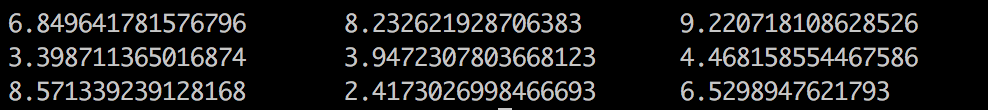
\includegraphics[width=0.9\textwidth]{centroids}
\caption{output centroids}
\label{fig: output centroids}
\end{figure}
 


 


%----------------------------------------------------------------------------------------
%\end{multicols}
\end{document}
